%------------------------------------------------
\begin{frame}
\frametitle{Encryption}
\justifying{
\begin{block}{Locally - your data}
\begin{itemize}
\item Hard disk
\item USB Key
\item Smartphone
\end{itemize}
\end{block}

\begin{block}{Network - Communications}
\begin{itemize}
\item Https : HTTPSEveryWhere for Firefox  
\item E-mails : GPG with Enigmail for Thunderbird
\item Connexion : VPN, SSH, TOR...
\end{itemize}
\end{block}

\begin{block}{}
$\Rightarrow$ Each "use", there is an encryption solution.
\end{block}
}
\end{frame}


%----------------------------------------------------------------------------------------
\begin{frame}
\frametitle{Emails - PGP, GPG?}
\begin{block}{PGP}
\justifying{
Pretty Good Privacy - PGP is an encryption software created by the American Phil Zimmermann in 1991.
}
\end{block}
\begin{block}{OpenPGP}
\justifying{
This standard describes the format of messages, signatures or certificates that can send software such as GNU Privacy Guard. It is therefore not a software but a format for the secure exchange of data, which owes its name to the historic program Pretty Good Privacy (PGP).
}
\end{block}
\begin{block}{GnuPG}
\justifying{GnuPG (GNU Privacy Guard) is the free software.}
\end{block}
\end{frame}


%----------------------------------------------------------------------------------------
\begin{frame}

\frametitle{Harddisk encryption}
\begin{block}{Software integrated in operating systems}
\begin{itemize}
\item Windows 7/8 : Bitlocker (Backdoor)
\item MacOS : FileVault
\item GNU/Linux : Encfs...
\end{itemize}
Can you trust closed source software ?
\end{block}

\begin{block}{Independently of the operating system}
$\Rightarrow$ TrueCrypt. For a USB key/an external hard drive.
\end{block}
\end{frame}

%----------------------------------------------------------------------------------------
\begin{frame}
\frametitle{TrueCrypt audit}
\begin{center}
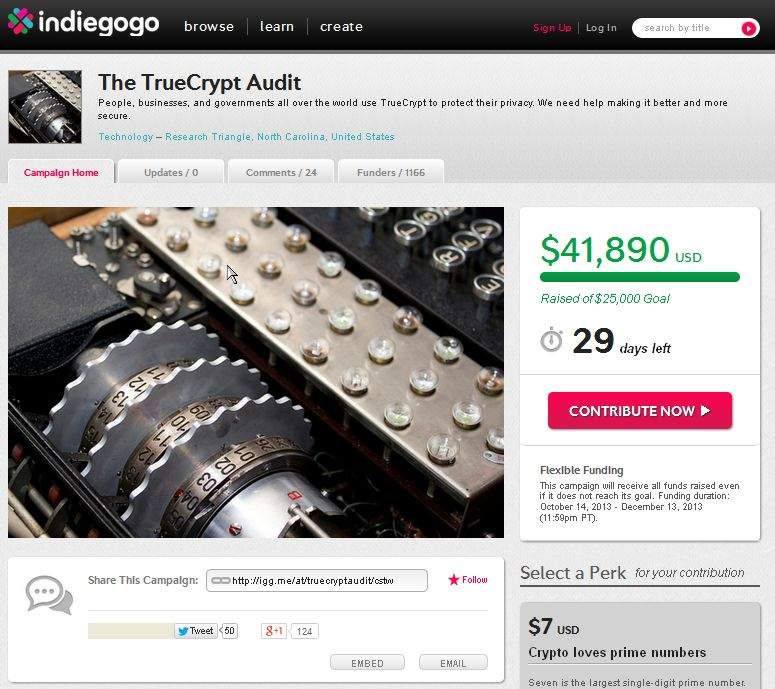
\includegraphics[scale=0.45] {./materials/truecryptaudit.jpg} 
\end{center}
\end{frame}

%----------------------------------------------------------------------------------------
\begin{frame}
\frametitle{Encryption and privacy}
\huge{Encryption is a need for privacy and allow data protection.}
\end{frame}
